%% 
%% Copyright 2019-2024 Elsevier Ltd
%% 
%% This file is part of the 'CAS Bundle'.
%% --------------------------------------
%% 
%% It may be distributed under the conditions of the LaTeX Project Public
%% License, either version 1.3c of this license or (at your option) any
%% later version.  The latest version of this license is in
%%    http://www.latex-project.org/lppl.txt
%% and version 1.3c or later is part of all distributions of LaTeX
%% version 1999/12/01 or later.
%% 
%% The list of all files belonging to the 'CAS Bundle' is
%% given in the file `manifest.txt'.
%% 
%% Template article for cas-dc documentclass for 
%% double column output.

\documentclass[a4paper,fleqn]{cas-sc}

\usepackage{subcaption}

\usepackage{multicol}

\usepackage[thinc]{esdiff} % for derivatives

% commands I use a lot
\usepackage{xspace}
\newcommand\thedata {$\{(t_i,h_{\text{obs}, i})\}_{i=1}^{N}$\xspace}
\newcommand\thedatanomath {\{(t_i,h_{\text{obs}, i})\}_{i=1}^{N}}
\newcommand\themodel {$h(t; h_0, \boldsymbol \alpha, \boldsymbol\theta)$\xspace}
\newcommand\themodelnomath {h(t; h_0, \boldsymbol \alpha, \boldsymbol\theta)}
\newcommand\thevars{h_0, \boldsymbol \alpha, \boldsymbol \theta, \sigma^2}

\usepackage{wrapfig}
% If the frontmatter runs over more than one page
% use the longmktitle option.

%\documentclass[a4paper,fleqn,longmktitle]{cas-dc}

%\usepackage[numbers]{natbib}
%\usepackage[authoryear]{natbib}
\usepackage[authoryear,longnamesfirst]{natbib}

%%%Author macros
\def\tsc#1{\csdef{#1}{\textsc{\lowercase{#1}}\xspace}}
\tsc{WGM}
\tsc{QE}
%%%

% Uncomment and use as if needed
%\newtheorem{theorem}{Theorem}
%\newtheorem{lemma}[theorem]{Lemma}
%\newdefinition{rmk}{Remark}
%\newproof{pf}{Proof}
%\newproof{pot}{Proof of Theorem \ref{thm}}


\begin{document}
\let\WriteBookmarks\relax
\def\floatpagepagefraction{1}
\def\textpagefraction{.001}

% Short title
\shorttitle{}    

% Short author
\shortauthors{}  

% Main title of the paper
\title [mode = title]{
Supporting Information: Scanning the cross-sectional area of a solid inside an opaque tank 
  via liquid level dynamics during draining
 }  

% Title footnote mark
% eg: \tnotemark[1]
\tnotemark[1] 

% Title footnote 1.
% eg: \tnotetext[1]{Title footnote text}
\tnotetext[1]{} 

% First author
%
% Options: Use if required
% eg: \author[1,3]{Author Name}[type=editor,
%       style=chinese,
%       auid=000,
%       bioid=1,
%       prefix=Sir,
%       orcid=0000-0000-0000-0000,
%       facebook=<facebook id>,
%       twitter=<twitter id>,
%       linkedin=<linkedin id>,
%       gplus=<gplus id>]

\author[1]{Gbenga Fabusola}%[<options>]

% Credit authorship
% eg: \credit{Conceptualization of this study, Methodology, Software}
\credit{}

% Address/affiliation
\affiliation[1]{organization={Oregon State University},
            % addressline={}, 
            city={Corvallis},
%          citysep={}, % Uncomment if no comma needed between city and postcode
            postcode={97331}, 
            state={Oregon},
            country={USA}}

\author[1]{Cory Simon}

% Footnote of the second author
\cormark[1]

% Email id of the second author


% URL of the second author
\ead[url]{}

% Credit authorship
\credit{}


% Corresponding author text
\cortext[2]{Corresponding author}

% Footnote text
\fntext[1]{}


\renewcommand{\abstract}{} % Extremely risky!
\begin{abstract}
\end{abstract}
% For a title note without a number/mark
%\nonumnote{}
% Keywords
\maketitle

\newpage 

\section{Geometry of the tank}

\begin{figure}[h!]
	\centering
	 \begin{subfigure}[b]{0.35\textwidth}
		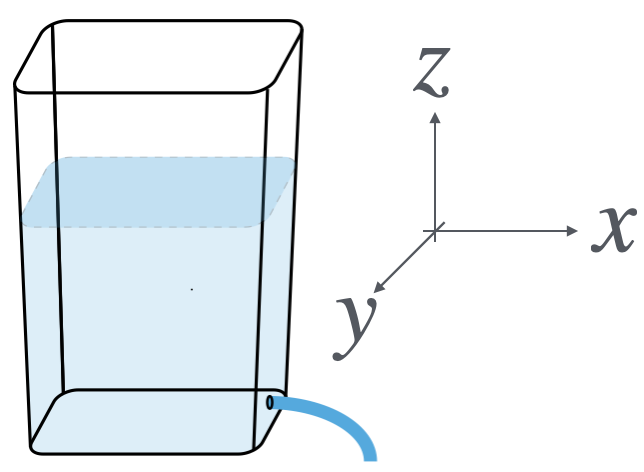
\includegraphics[width=\textwidth]{../drawings_and_photos/views.png} \caption{}
	\end{subfigure}
	
	\begin{subfigure}[b]{0.8\textwidth}
		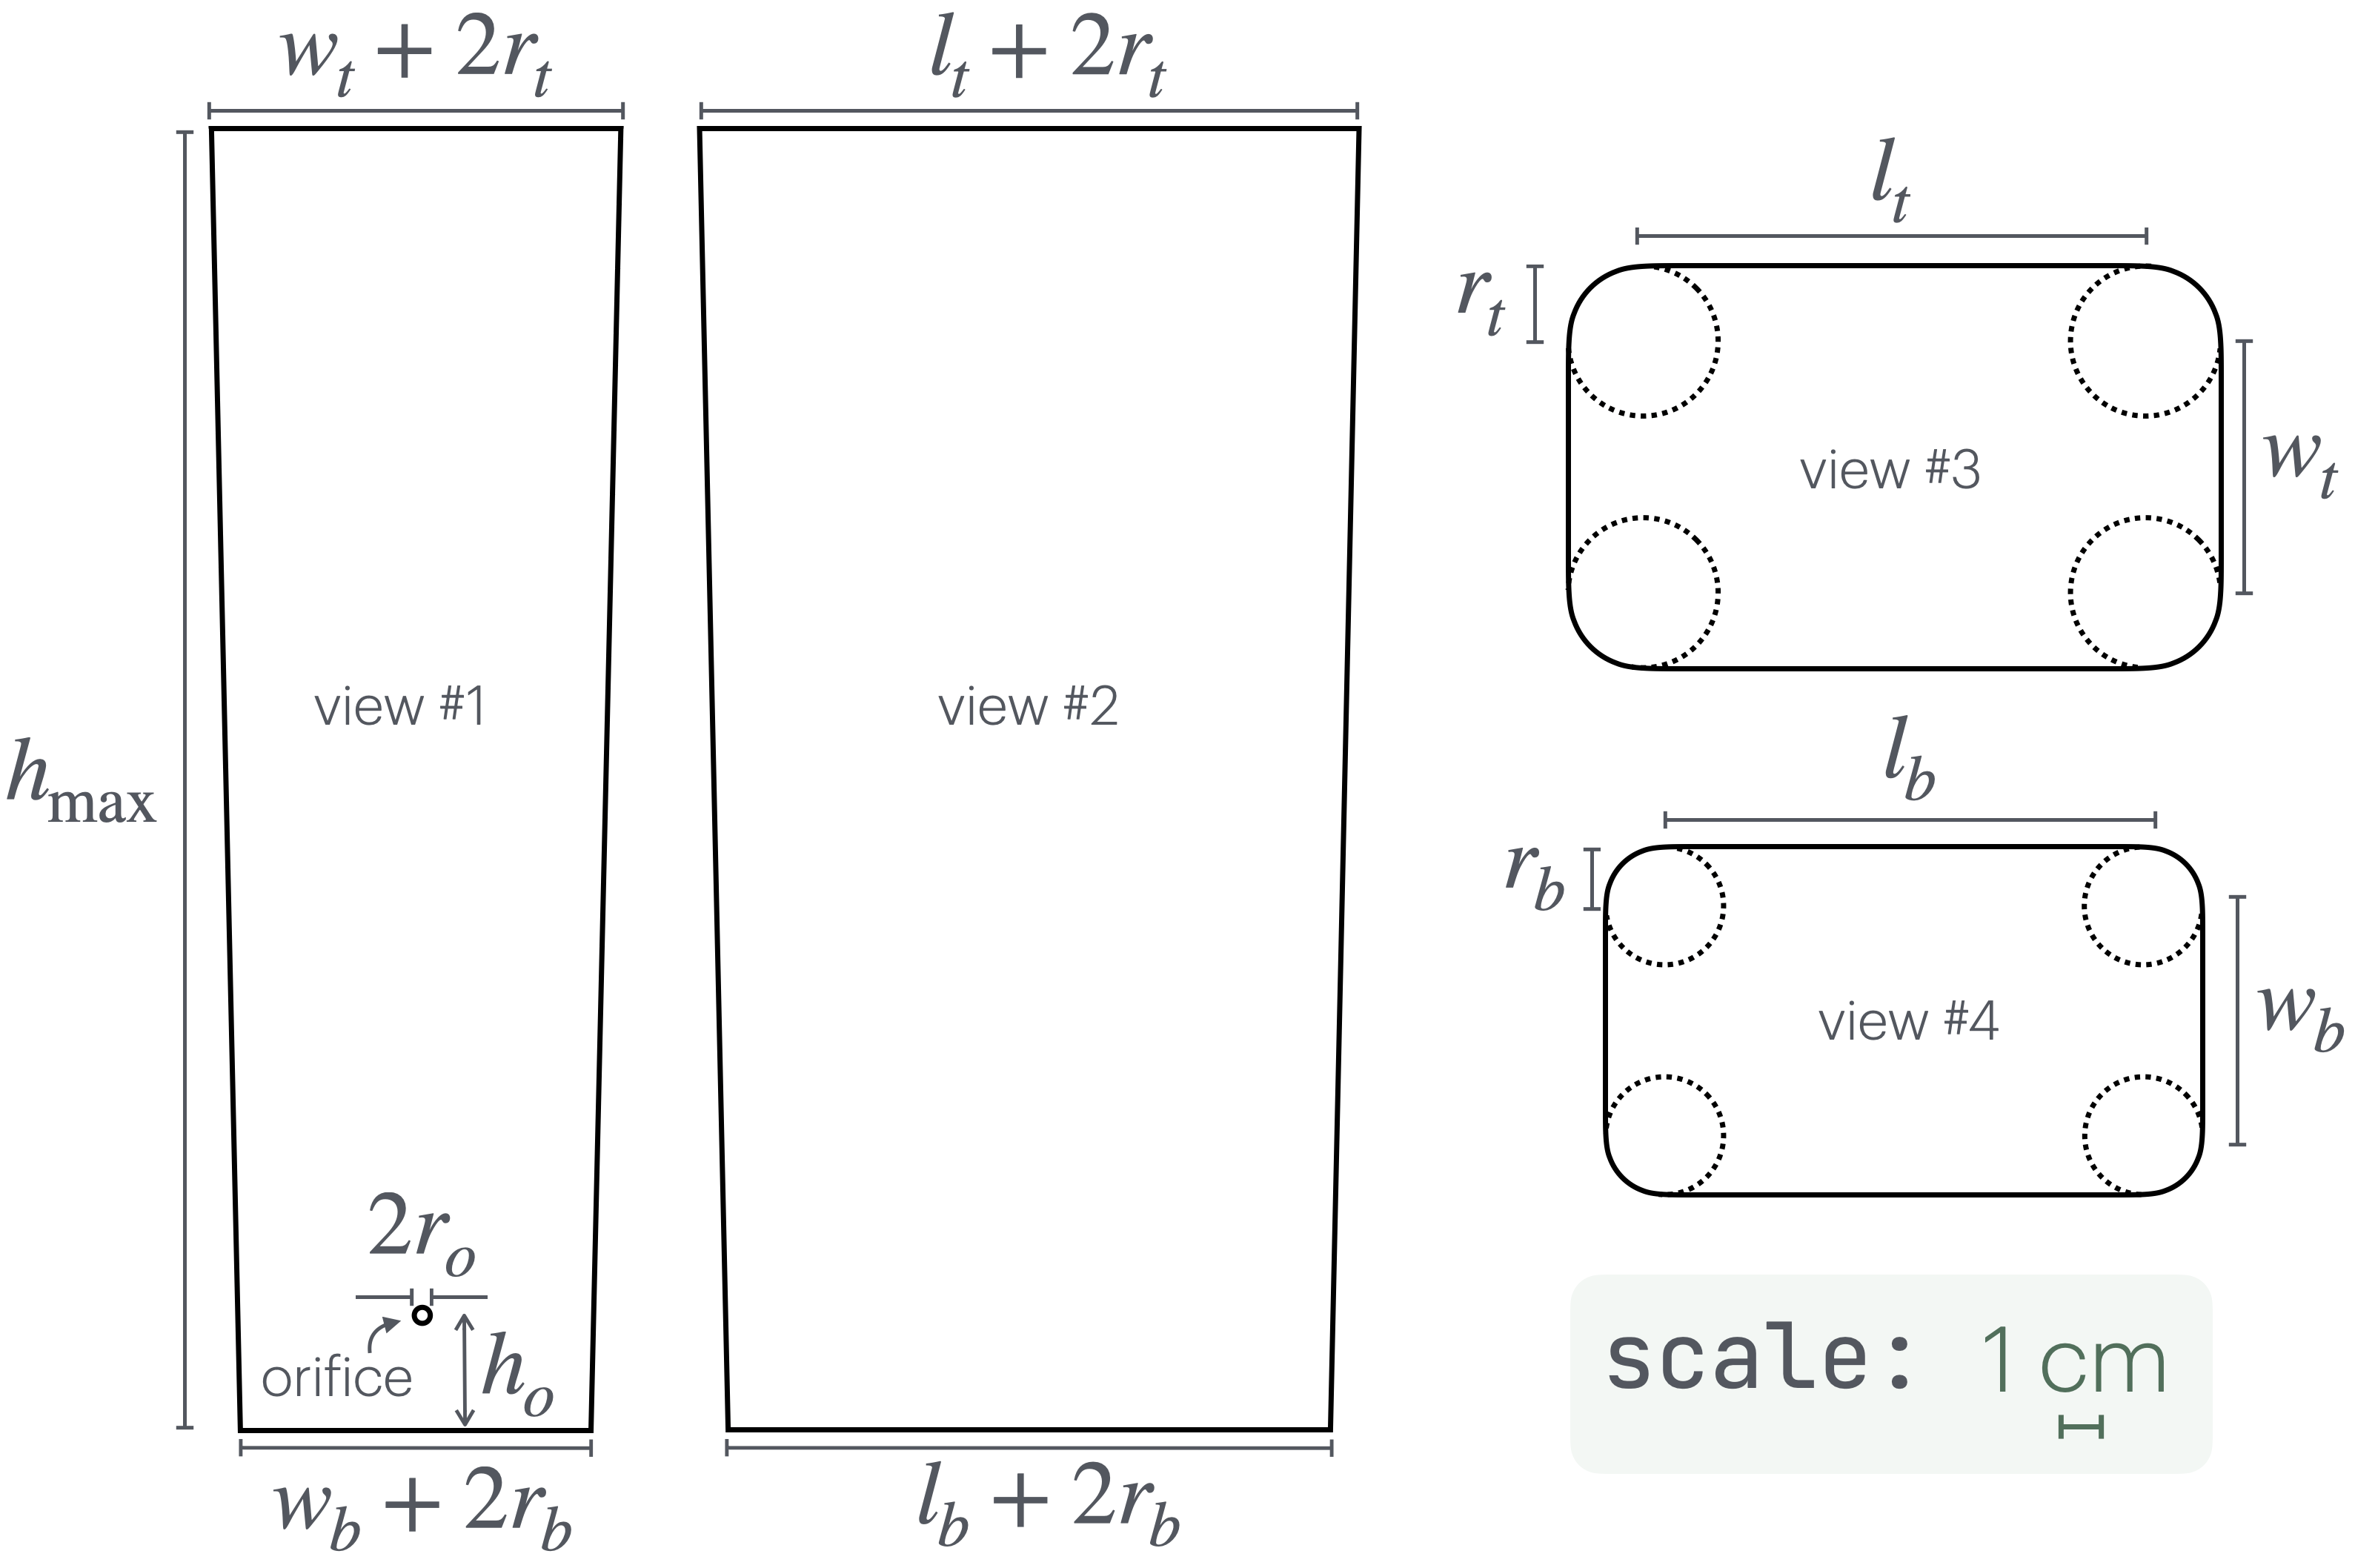
\includegraphics[width=\textwidth]{../drawings_and_photos/tank_geometry.png} \caption{}
	\end{subfigure}
	\caption{Geometry of our tank. 
	(a) The 3D geometry of the tank with a coordinate axes to define the views we show. (b) The tank from four views, drawn approximately to scale, with variables denoting the dimensions marked. Each cross-section of the tank, taken parallel with the ground, is a rounded rectangle.
	}
\end{figure}

\section{Cross-sectional area of the tank and solid contained in the tank}




\section{Obtaining Torricelli's Law from Bernoulli's Equation}

\begin{wrapfigure}{r}{0.35\textwidth}
	\centering
	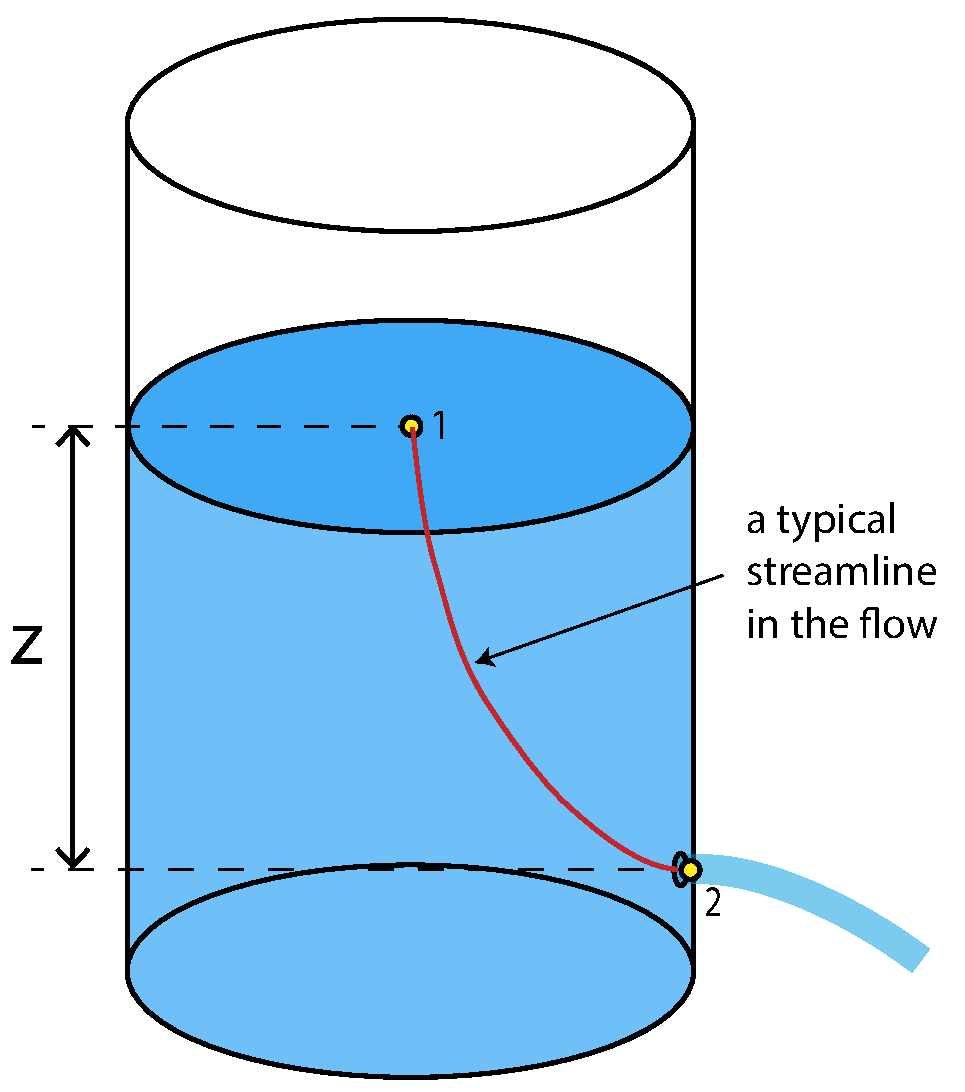
\includegraphics[width=0.35\textwidth]{../drawings_and_photos/torricelli_illustration.pdf}
	\caption{Applying Bernoulli's equation to points (1) and (2) along the typical flow streamline shown gives Torricelli's law after neglecting the small downward velocity of the liquid level in the tank. Sketch mimics Problem 3B.14 in Edition 2 of Bird, Stewart, and Lightfoot \cite{bsl_book}.}
\end{wrapfigure}

	Consider an open-top tank with a small hole in its side. Suppose we nearly fill the tank with liquid then allow liquid to flow out of the tank through the small hole, to the atmosphere. (This flow is driven by the force of gravity.)
	At some moment in time, let $z$ [m] be the height of the liquid above the center of the hole. 
	We wish to find the corresponding velocity $v_2$ [m/s] at which the liquid is ejecting from the side of the tank. 
	
	To do so, we follow Bird, Stewart, and Lightfoot \cite{bsl_book} (Problem 3B.14 in Edition 2) by applying Bernoulli's equation to two points in the liquid: 
	(1) a point just below the surface of the liquid at the top of the tank, near the center of the tank, and 
	(2) a point inside the outlet stream, just outside of the tank and near the center of the cross-section of the stream. 
	 Conceptually, we're considering a typical streamline of the flow extending from point (1) to point (2).
	We make three approximations about the liquid along this streamline: 
	(1) the flow is at steady-state, which applies the quasi-steady-state assumption that $z$ is approximately constant despite dropping slowly,
	(2) the liquid is inviscid (i.e., we neglect frictional forces internal to the liquid),
	and
	(3) the liquid is incompressible (i.e., its density, $\rho$ [kg/m$^3$], is constant).
	(Also, the flow is isothermal.)
	
	A mechanical energy balance then implies Bernoulli's equation \cite{welty2020fundamentals} holds for points (1) and (2) along the flow streamline, which relates the velocity $v_i$ [m/s], pressure $P_i$ [N/m$^2$ $[=]$ kg /(s$^2\cdot$m)], and elevation $y_i$ [m] of the liquid at the two points $i\in\{1,2\}$:
	\begin{equation}
	g y_1 + \frac{1}{2} v_1^2 + \frac{P_1}{\rho} = gy_2 + \frac{1}{2} v_2^2 + \frac{P_2}{\rho} 
	\end{equation}
	where $g$ [m/s$^2$] is the gravitational acceleration constant. 
	
	Now, since both the top of the tank and the stream ejecting from the side of the tank are open to the atmosphere, we have $P_1=P_2$ both at atmospheric pressure. And, we have $y_1-y_2=z$. Further, we approximate $v_1\approx 0$ since the cross-sectional area of the liquid at the top of the tank is large relative to the cross-sectional area of the hole in the side of the tank (making $v_2 >> v_1$). Bernoulli's equation then reduces to:
	\begin{equation}
	g z  = \frac{1}{2} v_2^2,
	\end{equation}
	which states that the decrease in gravitational potential energy of a parcel of liquid that traveled from point (1) to (2) matches its gain in kinetic energy. Solving for $v_2$ gives Torricelli's law \cite{driver1998torricelli}:
	\begin{equation}
	v_2 = \sqrt{2gz}.
	\end{equation}
	The velocity of the liquid ejecting from the side of the tank is proportional to the square root of the height of liquid $z$ above the hole. The gravitational acceleration constant appears because gravity is the force that drives the flow.
% Biography
%\bio{}
% Here goes the biography details.
%\endbio

%\bio{pic1}
% Here goes the biography details.
%\endbio

\clearpage

\bibliographystyle{elsarticle-num}

% Loading bibliography database
 \bibliography{refs}

\end{document}

